%%
%% This is file `mcmthesis-demo.tex',
%% generated with the docstrip utility.
%%
%% The original source files were:
%%
%% mcmthesis.dtx  (with options: `demo')
%%
%% -----------------------------------
%%
%% This is a generated file.
%%
%% Copyright (C)
%%       2010 -- 2015 by Zhaoli Wang
%%       2014 -- 2019 by Liam Huang
%%       2019 -- present by latexstudio.net
%%
%% This work may be distributed and/or modified under the
%% conditions of the LaTeX Project Public License, either version 1.3
%% of this license or (at your option) any later version.
%% The latest version of this license is in
%%   http://www.latex-project.org/lppl.txt
%% and version 1.3 or later is part of all distributions of LaTeX
%% version 2005/12/01 or later.
%%
%% This work has the LPPL maintenance status `maintained'.
%%
%% The Current Maintainer of this work is latexstudio.net.
%%
%%
%% This is file `mcmthesis-demo.tex',
%% generated with the docstrip utility.
%%
%% The original source files were:
%%
%% mcmthesis.dtx  (with options: `demo')
%%
%% -----------------------------------
%%
%% This is a generated file.
%%
%% Copyright (C)
%%       2010 -- 2015 by Zhaoli Wang
%%       2014 -- 2019 by Liam Huang
%%       2019 -- present by latexstudio.net
%%
%% This work may be distributed and/or modified under the
%% conditions of the LaTeX Project Public License, either version 1.3
%% of this license or (at your option) any later version.
%% The latest version of this license is in
%%   http://www.latex-project.org/lppl.txt
%% and version 1.3 or later is part of all distributions of LaTeX
%% version 2005/12/01 or later.
%%
%% This work has the LPPL maintenance status `maintained'.
%%
%% The Current Maintainer of this work is Liam Huang.
%%

\documentclass{mcmthesis}
\mcmsetup{CTeX = false,   % 使用 CTeX 套装时,设置为 true
        tcn = 2207690, problem = C,
        sheet = true, titleinsheet = true, keywordsinsheet = true,
        titlepage = false, abstract = true}
% \usepackage{newtxtext}%\usepackage{palatino}
\usepackage{tikz}
\usepackage{lipsum}
\usepackage{algorithm}
\usepackage{algorithmicx}
\usepackage{algpseudocode}
\usepackage{amsmath}
\usepackage{graphicx} %插入图片的宏包
\usepackage{float} %设置图片浮动位置的宏包
\renewcommand{\algorithmicrequire}{\textbf{Input:}}  
\renewcommand{\algorithmicensure}{\textbf{Output:}} % Use Output in the format of Algorithm
\title{Portfolio Arrangement}
\author{\small \href{https://www.latexstudio.net/}
  {\includegraphics[width=7cm]{mcmthesis-logo}}}
\date{\today}
\begin{document}
\begin{abstract}
Use this template to begin typing the first page (summary page) of your electronic report. This template uses a 12-point Times New Roman font. Submit your paper as an Adobe PDF electronic file (e.g. 1111111.pdf), typed in English, with a readable font of at least 12-point type.

Do not include the name of your school, advisor, or team members on this or any page.

Papers must be within the 25 page limit.

Be sure to change the control number and problem choice above.
You may delete these instructions as you begin to type your report here.

Follow us @COMAPMath on Twitter or COMAPCHINAOFFICIAL on Weibo for the most up to date contest information.

\begin{keywords}
keyword1; keyword2
\end{keywords}
\end{abstract}
\maketitle

Generate the Table of Contents, if it's needed.
\tableofcontents
\newpage

Generate the Memorandum, if it's needed.
\memoto{\LaTeX{}studio}
\memofrom{Liam Huang}
\memosubject{Happy \TeX{}ing!}
\memodate{\today}
\begin{memo}[Memorandum]
  \lipsum[1-3]
\end{memo}


\section{Introduction}
\subsection{Background of the problem}

 Investment in financial products is a common way to produce extra income and favorable profits.
This means the buy and sell of several products at a time,
which can be rather relatively stable ones such as national debt,
or volatile assets, for example, gold and bitcoin.
While investing can make profits, it can also carry certain risks,
especially when the product is relatively unstable.
To maximize the profit and minimize the risk of an investment,
traders usually invest in several products at a time
and decide the holdings of each asset based on actual market conditions.
In terminology, this method is called \textit{portfolio management}.

Portfolio management is the process of managing investments,
constantly rearranging a certain amount of funds into several products or assets,
aiming at maximizing profit and ensuring low market risks at the same time.
There have been several traditional methods to solve this problem,
which can be roughly classified into these four categories\cite{li2014online}:

\begin{itemize}
  \item \textbf{Follow the winner}\\
  maximize the portfolio's expected growth rate
  \item \textbf{Follow the loser}\\
  transfer the fund from \textit{winner} asset to \textit{loser} asset
  \item \textbf{Pattern Matching}\\
  predict future market distribution based on historical data
  \item \textbf{Meta-Learning}\\
  tbd
\end{itemize}

There're many algorithms that combine these methods with machine learning.
These algorithms are reliable in short-term prediction
but do not behave well in long-term prediction.
This is because the algorithms highly depends on their accuracy,
but the natural uncertainty of the market makes it hard to predict.

\subsection{Restatement of the problem}

Based on the historical gold and BTC price data,
develop a model that helps to determine the holdings of cash, gold, and bitcoin every single day.
To note, the daily trading strategy should only be made using the price data before that day.

The final target is to make maximum profit from the given 1,000 USD principal,
and predict how much it will become five years later, based on the formerly developed model.

% \subsection{Syntax (how to type \LaTeX\ commands --- these
%   are the rules)}

% \lipsum[3]
% \begin{itemize}
% \item the angular velocity of the bat,
% \item the velocity of the ball, and
% \item the position of impact along the bat.
% \end{itemize}
% \lipsum[4]
% \emph{center of percussion} [Brody 1986], \lipsum[5]

% \begin{Theorem} \label{thm:latex}
% \LaTeX
% \end{Theorem}
% \begin{Lemma} \label{thm:tex}
% \TeX .
% \end{Lemma}
% \begin{proof}
% The proof of theorem.
% \end{proof}

% \subsection{Other Assumptions}
% \lipsum[6]
% \begin{itemize}
% \item
% \item
% \item
% \item
% \end{itemize}

% \lipsum[7]

\section{Analysis of the Problem}

\subsection{Transaction Costs}

% 然而,在实际的市场中,往往不能忽略交易的手续费。在考虑手续费时,设计的投资策略必须有效预计未来资产价格的走势情况,如果在短时间内频繁交易,由于手续费的存在,整体盈利会被极大影响。

However, in the actual market, the transaction cost cannot be ignored. When considering the transaction cost, the designed investment strategy must effectively predict the future trend of asset prices. If there are frequent transactions in a short period of time, the overall profit will be greatly affected due to the existence of the transaction cost.

% 在现实中,Transaction cost通常来自于资产佣金,交易市场等机构会在交易时收取阶梯定价的手续费,这些手续费通常与买卖资产的市值正相关。这种自然的手续费是无法被正确衡量的。然而,我们的模型做了一些简单化的假设,假定手续费是按照资产交易的数额按照百分率收取的,并且买入和卖出的手续费一致。

In reality, transaction costs usually come from asset commissions. Institutions such as trading markets will charge tiered pricing fees during transactions. These fees are usually positively related to the market value of assets bought and sold. This natural fee cannot be measured correctly. However, our model makes some simplistic assumptions, assuming that fees are charged as a percentage of the amount traded on the asset, and that the fees for buying and selling are the same.

\section{Hypotheses}

\begin{itemize}
  \item \textbf{Market closure days}\\
  There are cases that data is missing in the gold price data given.
  It can be observed that this vacancy basically occurs on weekends
  and during holidays such as Christmas day and the days around.
  We assume such vacancies occur on and only on gold market closure days.
  In this case, gold cannot be traded and the gold price won't change.\\
  This does not apply for bitcoin market, which does not have closure days.
  \item \textbf{Trade at the end of the day}\\
  Price changes during the trading hours each day are not taken into consideration
  as there is no relevant data.
  We assume that the data given in the question is the \textit{closing price}
  (i.e. the price at the end of the trading hours),
  and our trade is made at that market closing time ideally.
  \item \textbf{Ignore market impact}\\
  The amount of funds we put into the market is very little
  compared to the total assets in the market.
  Thus, we assume that our actions have zero effect on the market itself.
  \item \textbf{Instant trading}\\
  Transactions in the market are fast enough to be considered immediate.
  This allows us to take out or put in money once we make a trade, with no delay.
\end{itemize}

% \begin{figure}[h]
% \small
% \centering
% \includegraphics[width=8cm]{example-image-a}
% \caption{The name of figure} \label{fig:aa}
% \end{figure}

% \lipsum[8] \eqref{aa}
% \begin{equation}
% a^2 \label{aa}
% \end{equation}

% \[
%   \begin{pmatrix}{*{20}c}
%   {a_{11} } & {a_{12} } & {a_{13} }  \\
%   {a_{21} } & {a_{22} } & {a_{23} }  \\
%   {a_{31} } & {a_{32} } & {a_{33} }  \\
%   \end{pmatrix}
%   = \frac{{Opposite}}{{Hypotenuse}}\cos ^{ - 1} \theta \arcsin \theta
% \]
% \lipsum[9]

% \[
%   p_{j}=\begin{cases} 0,&\text{if $j$ is odd}\\
%   r!\,(-1)^{j/2},&\text{if $j$ is even}
%   \end{cases}
% \]

% \lipsum[10]

% \[
%   \arcsin \theta  =
%   \mathop{{\int\!\!\!\!\!\int\!\!\!\!\!\int}\mkern-31.2mu
%   \bigodot}\limits_\varphi
%   {\mathop {\lim }\limits_{x \to \infty } \frac{{n!}}{{r!\left( {n - r}
%   \right)!}}} \eqno (1)
% \]

\section{Vector autoregression model}

\subsection{Introduction to the model}
It is a general approach to make regressing from past price dates and forecasting a period price. Then design an algorithm to make a plan for rearranging the ratio of assets. These methods can be classified as ``two-staged methods''.

Vector autoregression model is a highly recognized time series analysis model. In previous research, vector autoregression model has been widely used in investment management, quantitative trading and so on. These models usually model the existing data, and then select the last piece of data for prediction and comparison as a reference. The autoregressive model has been shown to have very good interpolation accuracy and can also accurately predict the development trend in the next few days in terms of prediction.


\subsection{Model building}

Out of all the bitcoin price data, our model is trained on data except the last seven days to get the last seven days of bitcoin price data. Then use these price data to compare with the actual price to judge whether the prediction is reasonable. Before this judgment, the correlation coefficient must be determined. If the correlation coefficient is not high enough, the autoregressive model cannot be solved.
An workflow of the autoregressive model is shown in figure \ref{AR}.

\begin{itemize}
  \item \textbf{Determine whether the data is stationary}\\
  The autoregressive model can only be applied to predict economic phenomena related to its own previous period (also known as its data stationary/weak stationary), such as economic phenomena that are greatly affected by its own historical factors, the mining volume of mines, the output of various natural resources etc.For economic phenomena that are greatly affected by social factors, autoregressive models are not suitable. Therefore, before establishing an autoregressive model, we first need to judge whether the subject conditions meet the requirements for establishing an autoregressive model.\\
  First of all ,formulate the null hypothesis $H_0$ :There is a unit root/UNIT ROOT (that is, the data is not stationary).\\
  % 存在单位根/UNIT ROOT(即数据不平稳)
  % 自回归模型只能适用于预测与自身前期相关的经济现象(也称作其数据平稳/弱平稳),例如受到自身历史因素影响较大的经济现象,如矿的开采量,各种自然资源产量等;对于受到社会因素影响较大的经济现象,不宜采用自回归模型。因此,在建立自回归模型之前,我们首先需要判断一下题目条件是否符合自回归模型的建立要求
  By using \textit{Augmented Dickey-Fuller Test},we can get the following results(three decimal places):\\
  \begin{table}[H]
    \centering
    \begin{tabular}{@{}lr@{}}
      \toprule
      Name & Value \\
      \midrule
      Statistical values & -0.238 \\
      P-value & 0.934 \\
      lags & 24.000 \\
      nobs & 1801.000 \\
      Threshold value(1\%) & -3.434 \\
      Threshold value(5\%) & -2.863 \\
      Threshold value(10\%) & -2.568 \\
      \bottomrule
    \end{tabular}
  \end{table}
  In the form:\textit{Statistical values}, \textit{P-value} and \textit{lags} are all statistical values obtained under the AIC standard, and the fisrt parameter is used for comparison with the lower 1\%, 5\%, and 10\% cutoffs.The second parameter represents the probability that the null hypothesis holds.The parameter \textit{nobs} is the number of observations used in this detection. The parameter maxlag in \textit{ADF TEST} is determined by it, and the formula is $ \displaystyle maxlag = 12 \times ( \frac{nobs}{100}) ^\frac{1}{4} $ .

  It can be seen from the \textit{P-value} that the probability of the null hypothesis is extremely low, thus we can reject the null hypothesis $H_0$, and the data is stationary.
  % 由p值可以看出,原假设成立的概率极底,我们应该拒绝原假设。即数据平稳

  \item \textbf{Quickly see if the data fits the AR model}\\
  According to the autoregressive function: \[ \hat{y_t} = b_0 + b_1 \times y_{t - 1} + \ldots + b_n \times y_{t - n} \qquad n < t \]
  We can determine whether $ y_{t + 1}$ and $ y_t $ are clearly related the picture\ref{fig:Figure_2} drawn by the computer.Also, we can calculate that the correlation coefficient is about 0.998 and the significance level is 0.0.

  \begin{figure}[h]
    \centering
    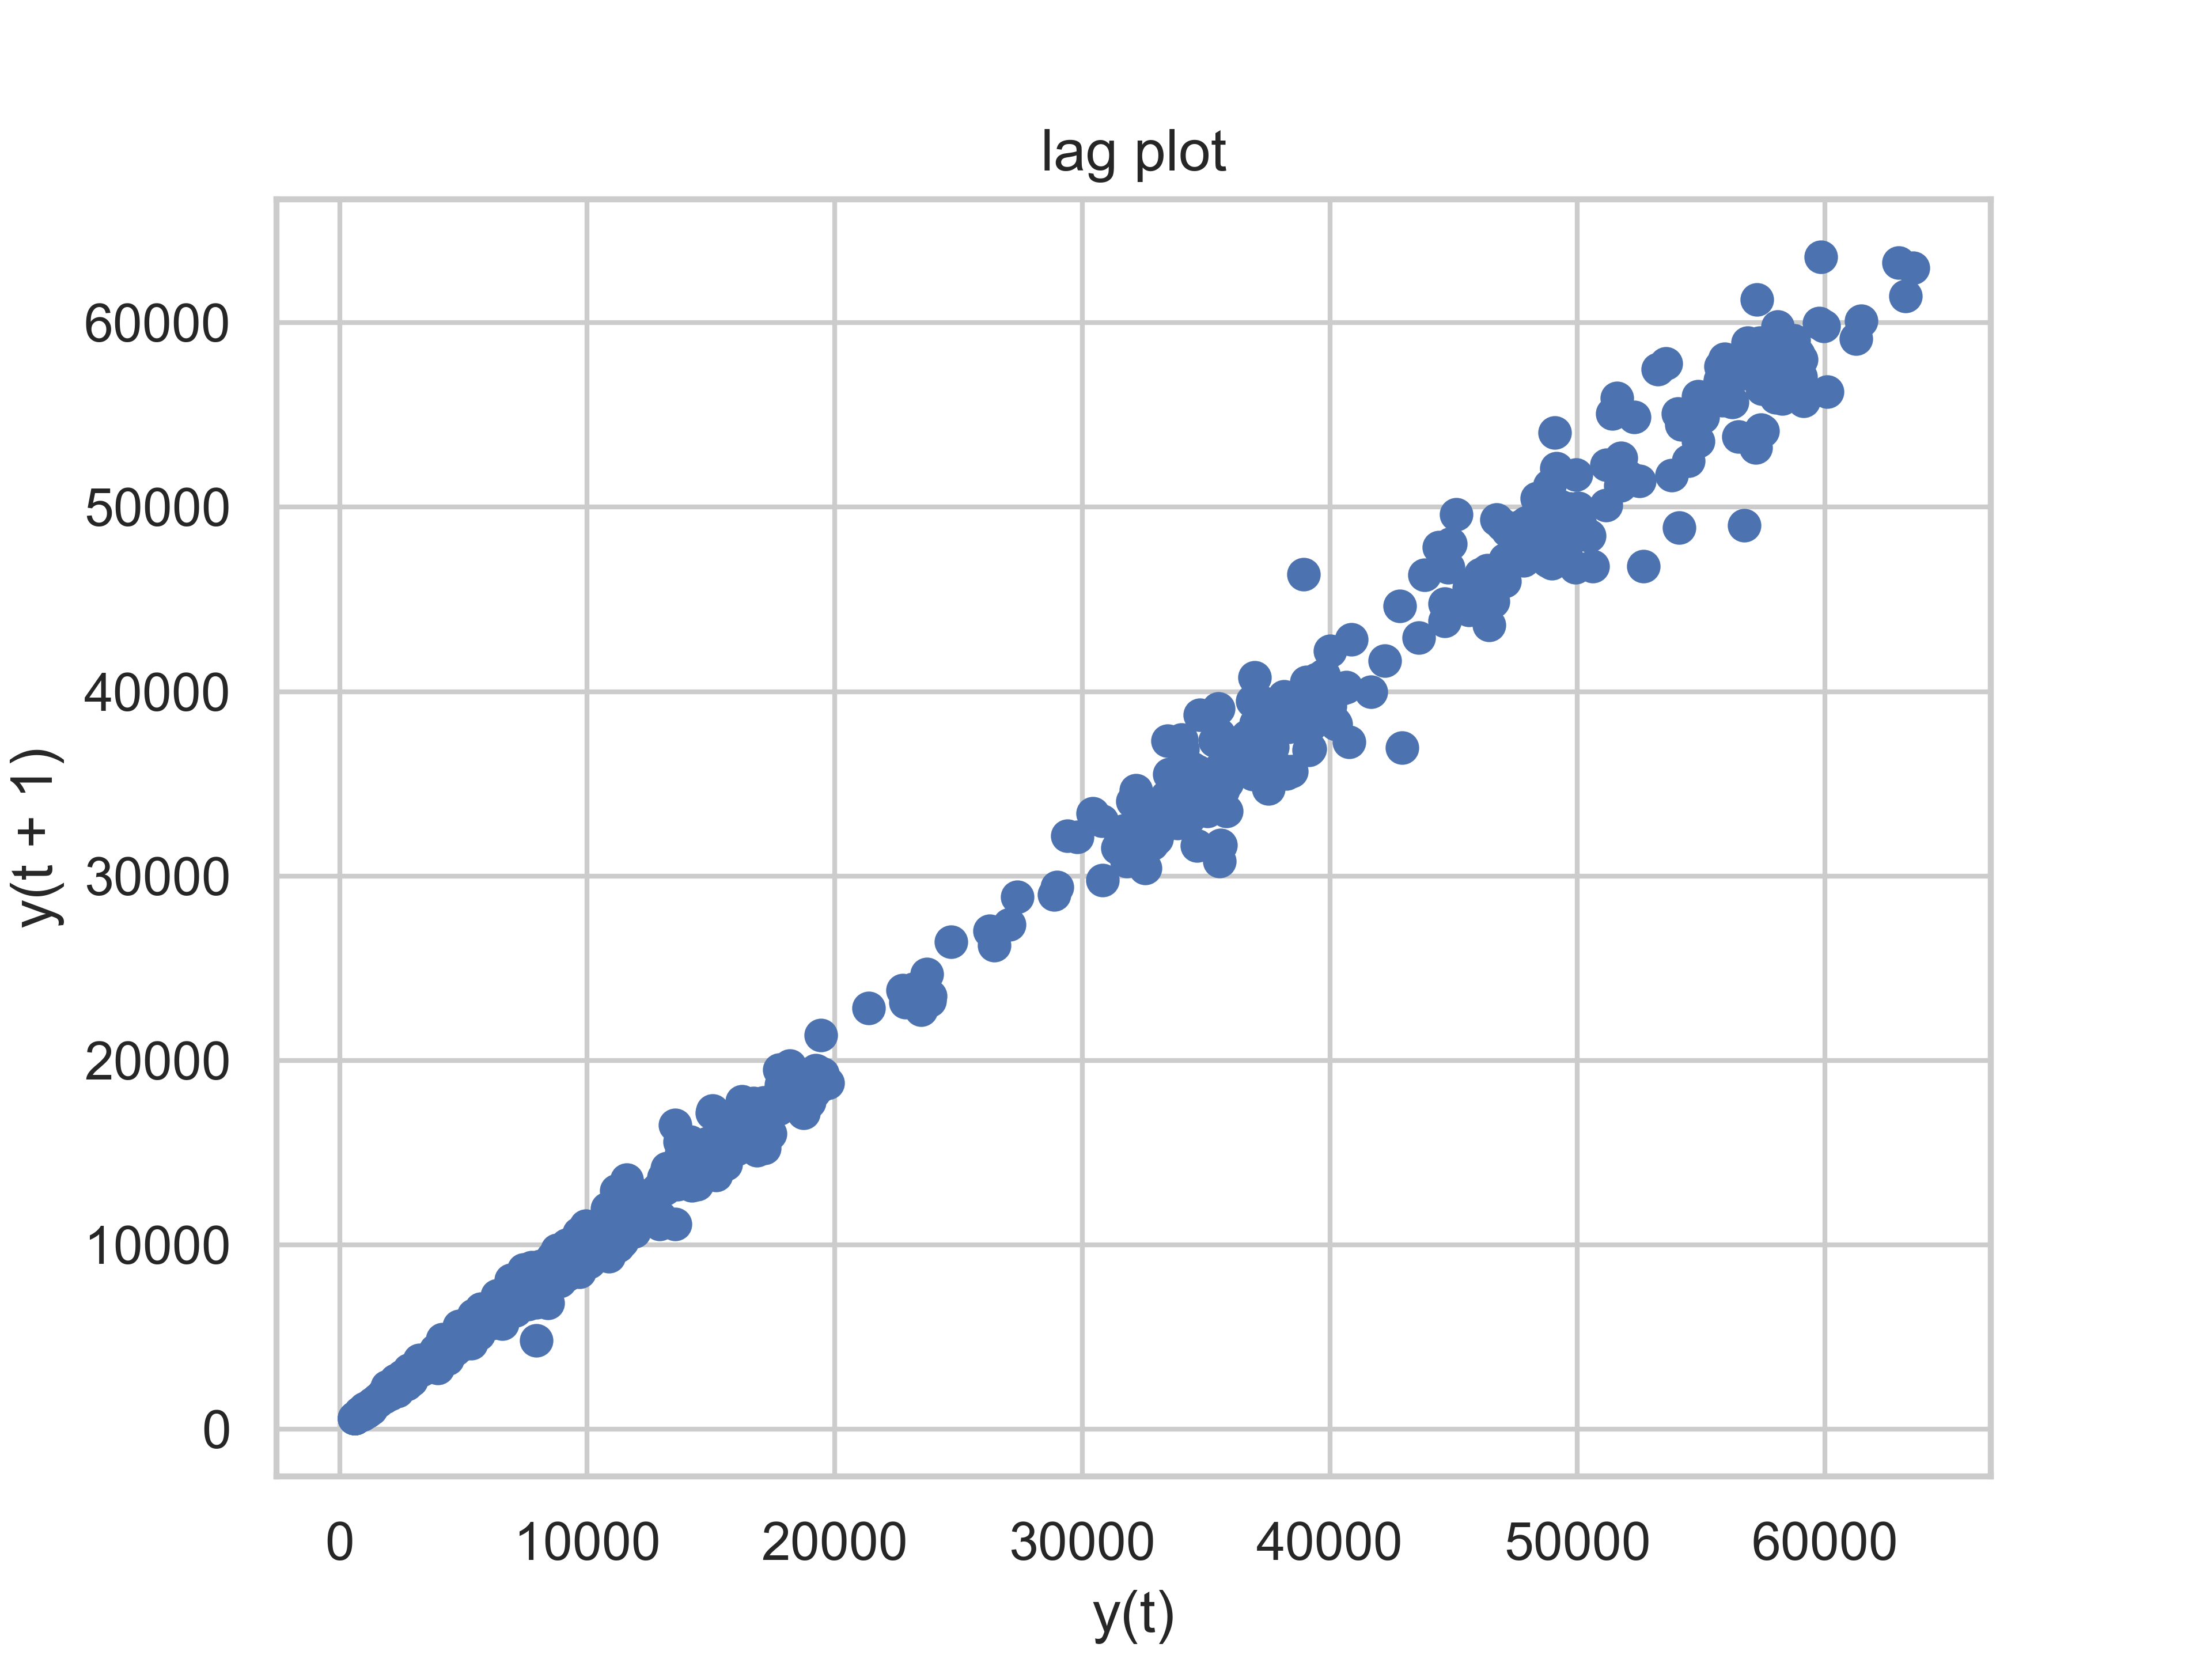
\includegraphics[width=0.5\textwidth]{lag_plot}
    \caption{Figure2}
    \label{The lag plot of correlation}
  \end{figure}
  \item \textbf{Ignore market impact}\\
 
  \item \textbf{Instant trading}\\
  
\end{itemize}

\begin{figure}[h]
  \tikzset{every picture/.style={line width=0.75pt}} %set default line width to 0.75pt

  \begin{tikzpicture}[x=0.75pt,y=0.75pt,yscale=-1,xscale=1]
  %uncomment if require: \path (0,300); %set diagram left start at 0, and has height of 300

  %Straight Lines [id:da8112233976325808]
  \draw    (100,101) -- (544,101) ;
  \draw [shift={(546,101)}, rotate = 180] [color={rgb, 255:red, 0; green, 0; blue, 0 }  ][line width=0.75]    (10.93,-3.29) .. controls (6.95,-1.4) and (3.31,-0.3) .. (0,0) .. controls (3.31,0.3) and (6.95,1.4) .. (10.93,3.29)   ;
  %Straight Lines [id:da7920278133084296]
  \draw    (512,65) -- (512,137) ;
  %Curve Lines [id:da46433491372617774]
  \draw    (265,124) .. controls (255.1,176.47) and (360.85,241.68) .. (401.78,213.87) ;
  \draw [shift={(403,213)}, rotate = 143.13] [color={rgb, 255:red, 0; green, 0; blue, 0 }  ][line width=0.75]    (10.93,-3.29) .. controls (6.95,-1.4) and (3.31,-0.3) .. (0,0) .. controls (3.31,0.3) and (6.95,1.4) .. (10.93,3.29)   ;
  %Curve Lines [id:da102775317135267]
  \draw    (566,208) .. controls (605.8,178.15) and (637.68,116.62) .. (571.01,88.42) ;
  \draw [shift={(570,88)}, rotate = 22.38] [color={rgb, 255:red, 0; green, 0; blue, 0 }  ][line width=0.75]    (10.93,-3.29) .. controls (6.95,-1.4) and (3.31,-0.3) .. (0,0) .. controls (3.31,0.3) and (6.95,1.4) .. (10.93,3.29)   ;

  % Text Node
  \draw (519,70) node [anchor=north west][inner sep=0.75pt]   [align=left] {7 days};
  % Text Node
  \draw (245,74) node [anchor=north west][inner sep=0.75pt]   [align=left] {Training data};
  % Text Node
  \draw (411,195) node [anchor=north west][inner sep=0.75pt]   [align=left] {Autoregression Model};
  % Text Node
  \draw (551,157) node [anchor=north west][inner sep=0.75pt]   [align=left] {predict};

  \end{tikzpicture}

  \caption{Autoregression model}
  \label{AR}
\end{figure}

\subsection{The Model Results}


\subsection{Model summary}



\section{Reinforcement learning model}

As concluded before,
the method of predicting with VAR is straightforward,
but still not accurate enough.
Thus, this section presents one possible solution using the Reinforcement learning (RL) model,
trying to improve the algorithm accuracy.

\subsection{Introduction to reinforcement learning}

\subsubsection{Deep learning}

Deep learning is part of machine learning and also part of artificial intelligence,
based on artificial neural networks, or ANN.
ANN is inspired by the biological neural network
and shares a similar structure with it, as diagram[\ref{ANN}] shows:

\begin{figure}[h]
\small
\centering
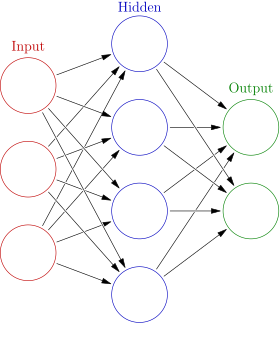
\includegraphics[width=5cm]{Colored_neural_network.svg.png}
\caption{Artificial neural network} \label{ANN}
\end{figure}

An ANN is based on a collection of connected units or nodes called artificial neurons,
which corresponds to the concept of neurons in a biological brain.
The connections between these nodes are called \textit{edges}.
They can transmit signals from one node to another,
just like what synapses in a biological brain do.
Inside each node, the data from the previous node is calculated in a non-linear way
and passed on to the next node.

The 'deep' in deep learning refers to the use of multiple layers in ANN.
Nodes in NAA are divided into several layers,
and different layers might perform different transformations on the input data.
The very first layer is called the input layer and,
accordingly, the last layer is referred to as the output layer.
Those layers between the first and the last layer are called \textit{hidden} layers.

Deep learning can be divided into three categories.
The learning is rather supervised, semi-supervised, or unsupervised.
Every neuron and edge has a \textit{weight} that can be adjusted in the learning process.
Given sample \textit{observations}, NAA adjusts the weight of the nodes and edges,
trying to improve the accuracy of the output.
This process is done by lowering the observed error rate.
In this case, learning won't stop until
extra observations don't efficiently reduce the error rate.

\subsubsection{Reinforcement learning}

 Reinforcement learning is a field of deep learning.
Diagram[\ref{LA}] shows the basic elements of reinforcement learning:

\begin{figure}[h]
  \small
  \centering
  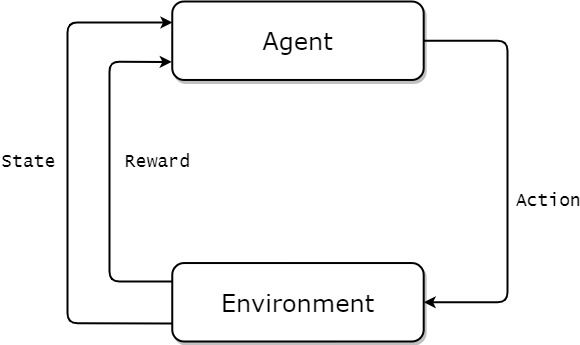
\includegraphics[width=9cm]{RL.jpg}
  \caption{Reinforcement learning} \label{LA}
\end{figure}

In a reinforcement learning model, there is one \textit{agent},
who performs as a learner or decision-maker.
\textit{Actions} of the agent influences the \textit{environment}.
In turn, the environment determines the \textit{state} of the learner
and gives the learner a certain amount of \textit{reward}.
It's kinda like a game, where players take their actions and get a relevant award from the system.
Players will continuously change their actions to maximize their rewards.

A reinforcement learning model works just like that,
but there is no game guides it can refer to --
all given to the model is some ``in-game data''.
Reinforcement learning does not require a large quantity of data to feed,
as supervised learning and unsupervised learning do.
Briefly, reinforcement learning is a ``trial and error'' approach to learning,
interacting constantly with the environment to gain feedback and
adjust behavior for maximum reward.

\subsubsection{Markov decision process}

 The process studied by deep learning is usually normalized as a \textit{Markov decision process}, or MDP.
MDPs are defined to have \textit{Markov property}:

\begin{itemize}
  \item The future can be fully predicted only using \textit{present} states;
  \item The future does not depend on the \textit{past};
  \item The past does not \textit{directly} effect the future.
\end{itemize}

In one word, Markov property refers to the memoryless property of a process, or

\begin{equation}
  P(s_{t+1}\vert s_t) = P(s_{t+1}\vert s_t,...,s_2,s_1).
\end{equation}

A stochastic and continuous decision-making process with Markov property
is called a Markov decision process.
A MDP can be described as a 4-tuple:

\begin{equation}
(\pmb{S},\pmb{A},\pmb{P},\pmb{R})
\end{equation}

\begin{itemize}
  \item $\pmb{S}$ is the set of states, called the state space;
  \item $\pmb{A}$ is the set of actions, called the action space;
  \item $\pmb{P}_a(s_t, s_{t+1})$ is the probability that action $a$ in state $s_t$ on day $t$ will lead to state $s_{t+1}$ on day $t+1$;
  \item $\pmb{R}_a(s_t, s_{t+1})$ is the expected reward received on day $t+1$, based on state $s_t$ and action $a$ on day $t$.
\end{itemize}

These elements make the foundation of MDPs.
A simplified MDP is shown in diagram[\ref{MDP}].

\begin{figure}[h]
  \small
  \centering
  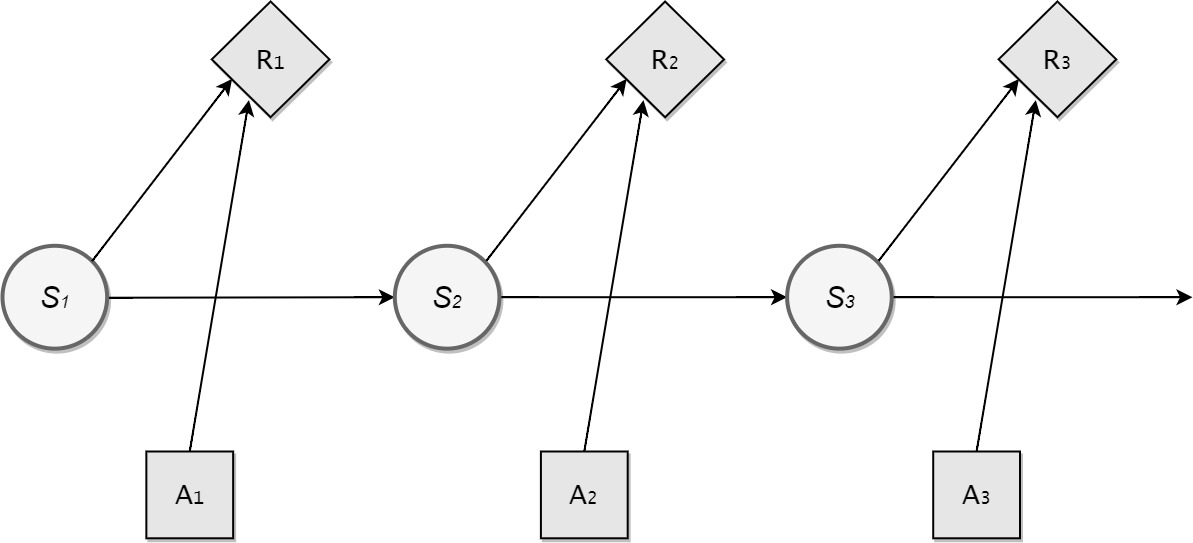
\includegraphics[width=11cm]{MDP.jpg}
  \caption{Markov decision process} \label{MDP}
\end{figure}

With all these $\pmb{A}$s and $\pmb{R}$s,
the goal is abstracted as finding an exact way to decide all the $a_t$
to maximize the final reward.
This reward is the combination of all the $\pmb{R}$s.
In most cases, it represents the mathematical expectation of the sum of $\pmb{R}$s,
$E(\Sigma R)$.

\subsubsection{Proximal policy optimization}

Proximal policy optimization (PPO) is a policy gradient method for reinforcement learning.

tbd

\subsection{Data Treatments}

% 在给出的数据表中,黄金的的价格数据有所缺失,as mentioned above,这是由于黄金在一些特殊的日期会停止交易。我们的模型将日期补齐,并将黄金的数据和比特币的数据根据日期作对齐处理。

% 注意到,这个过程会将黄金的缺失数据填充为NAN,即Not A Number,我们的模型对黄金的缺失数据有特别的处理,这会在后文的叙述中给出说明。

In the data table given, the price data for gold is missing, as mentioned above, this is due to the fact that gold stops trading on some special dates. Our model pads the date and aligns the gold data and bitcoin data according to the date.

Note that this process will fill in the missing data of gold as NAN, that is, Not A Number. Our model has a special treatment for the missing data of gold, which will be explained in the following description.


\subsection{Model building}

This part presents a solution based on Reinforcement learning,
using a \textbf{proximal policy optimization} algorithm.

\subsubsection{The environment, agent and state}

The \textit{environment} represents the market itself,
which contains all the data needed.
Here the environment can be simply described
by the current and historical price of gold and bitcoin.
The \textit{agent} is the reinforcement learning algorithm which
continuously trades in the environment.

The \textit{state} on day $t$, $s_t = (\pmb{w}_t, \pmb{p}_t, \rho _t)$, is made up of three parts:

\begin{itemize}
  \item $\pmb{w}_t = (w_1, w_2, w_3)$, or the weight vector \\is a 3-tuple.
  It describes the allocation of three types of assets.
  The three elements in $\pmb{w}$ stands for the percentage of cash, gold and bitcoin respectively,
  and it's clear that the sum of these percentages ($w_1+w_2+w_3$) is equal to 1.\\
  All our assets were held in cash at the very beginning,
  which means that regardless of the actions afterwards,
  $\pmb{w}$ is a $(1,0,0)$ at this special time.

  \item $\pmb{p}_t = (p_1, p_2, p_3)$, or the price vector \\ is also a 3-tuple,
  which represents current prices of the assets.
  Similarly, the three elements in $\pmb{p}$ corresponds to cash, gold and bitcoin.
  The "price" of cash is bound to be 1,
  so $\pmb{p}$ can be expressed in the form $(1,p_2,p_3)$.

  \item $\rho _t$\\
  stands for the total amount of funds we hold on day $t$.
  $\rho _t$ is the sum of current cash holdings and the market value of gold and bitcoin.
  According to this definition, $\rho _1$ on day 1 is 1000\$.
\end{itemize}

\subsubsection{The action and the reward}

\textit{Actions} are what the agent performs.
What an action $a_t$ does is to effect the state $s_t$ on day $t$
and change it to state $s_{t+1}$ on day $t+1$,
producing \textit{rewards} $r_t$ in the process.
In the case of our RL model,
$\pmb{p}$ is determined by the actual market data and influenced by actions,
according to the zero market impact hypothesis.
Also, $\rho $ is calculated afterwards using previous data.
Only $\pmb{w}$ is effected directly by actions.
The way in which actions affect the state is shown in graph[\ref{action}]:

\begin{figure}[h]
  \centering
  \tikzset{every picture/.style={line width=0.75pt}} %set default line width to 0.75pt

  \begin{tikzpicture}[x=0.75pt,y=0.75pt,yscale=-1,xscale=1]
      \draw    (75,164) -- (592,164) ;
      \draw [shift={(594,164)}, rotate = 180] [color={rgb, 255:red, 0; green, 0; blue, 0 }  ][line width=0.75]    (10.93,-3.29) .. controls (6.95,-1.4) and (3.31,-0.3) .. (0,0) .. controls (3.31,0.3) and (6.95,1.4) .. (10.93,3.29)   ;
      \draw    (100,125) -- (100,200) ;
      \draw    (524,126) -- (524,201) ;
      \draw    (118,137) -- (509,137) ;
      \draw [shift={(511,137)}, rotate = 180] [color={rgb, 255:red, 0; green, 0; blue, 0 }  ][line width=0.75]    (10.93,-3.29) .. controls (6.95,-1.4) and (3.31,-0.3) .. (0,0) .. controls (3.31,0.3) and (6.95,1.4) .. (10.93,3.29)   ;
      \draw (84,102.4) node [anchor=north west][inner sep=0.75pt]    {$\rho _{t}$};
      \draw (585,178) node [anchor=north west][inner sep=0.75pt]   [align=left] {Time};
      \draw (517,102.4) node [anchor=north west][inner sep=0.75pt]    {$\rho _{t+1}$};
      \draw (181,113.5) node [anchor=north west][inner sep=0.75pt]    {$\boldsymbol{w}_{t}$};
      \draw (413,113.4) node [anchor=north west][inner sep=0.75pt]    {$\boldsymbol{w}_{t+1}$};
      \draw (96,209) node [anchor=north west][inner sep=0.75pt]   [align=left] {$\displaystyle t$};
      \draw (510,206.4) node [anchor=north west][inner sep=0.75pt]    {$t+1$};
  \end{tikzpicture}

  \caption{An action of the agent} \label{action}
\end{figure}

The action done between day $t$ and day $t+1$ changes $\pmb{w}_t$ to $\pmb{w}_{t+1}$,
effecting $\rho $ in the process.
Total funds $\rho _{t+1}$ is calculated using
$\rho _t$, $\pmb{w}_t$, $\pmb{w}_{t+1}$, $\pmb{p}_t$ and $\pmb{p}_{t+1}$,
by the algorithm to be described in the next part.

Finally, the reward $r$ is used to show the growth rate of the total funds $\rho$:

\begin{equation}
  r_{t+1} = \log(\frac{\rho _{t+1}}{\rho _t} ).
\end{equation}

\subsubsection{The algorithm}

To calculate $\rho _{t+1}$ which is mentioned in last part,
we introduce a new variable $\pmb{A}_t$:

\begin{equation}
  \pmb{A}_t = (\rho _t \cdot \pmb{w}_t) \, \oslash \, \pmb{p}_t ,
\end{equation}

where $\oslash$ is the element-wise division operator.
$\pmb{A}_t$ is also a 3-tuple.
It indicates how many \textit{units} of holdings the agent holds on day $t$,
based on all the elements of the current state:
total amount of fund $\rho_t$, the allocation of assets $\pmb{w}_t$,
and the current market price $\pmb{p}_t$.
We can express the change in holdings in terms of the amount of change in $\pmb{A}$ ($\Delta \pmb{A}$).
For one certain asset,
a positive or negative $\Delta A$ corresponds to the agent buying or selling the asset respectively.

According to the question, a commission must be paid after each transaction is done,
$1\%$ for gold and $2\%$ for bitcoin.
A new vector $\pmb{c}$ is introduced to store this information,
$\pmb{c} = (0, 0.01, 0.02)$.

The formulae used when buying and selling differ when taking $\pmb{C}$ into account.
For those products that we buy (i.e. $\Delta A > 0$),
the amount spent on the purchase is greater than the actual value of the purchase,
which is $c\%$ less than the former.
The actual amount spent on day $t+1$ can be calculated using equation (\ref{buy-in}).

\begin{equation}
  \frac{p_{t+1} \cdot \Delta A_{t+1}}{1-c}
  = \frac{\rho _{t+1} \cdot w_{t+1} - \rho _t \cdot w_t \cdot (p_{t+1} / p_t)}{1-c}
  \label{buy-in}
\end{equation}

In the numerator,
$\rho _{t+1} \cdot w_{t+1}$ is the value on day $t+1$ after the trade,
and the second part $\rho _t \cdot w_t \cdot (p_{t+1} / p_t)$
is the value on day $t+1$ before the trade.
Thus, the difference represents the change in value caused by the transaction on day $t+1$,
and the expression stands for the amount of funds the agent actually spent
to cause that change.
% The numerator, $p_{t+1} \cdot \Delta A_{t+1}$,
% is the ideal amount spent on the buy-in when there is no commission.
Similarly, the formula for the asset that we sell (i.e. $\Delta A < 0$) is:

\begin{equation}
  p_{t+1} \cdot \Delta A_{t+1} \cdot (1 - c)
  = (\rho _{t+1} \cdot w_{t+1} - \rho _t \cdot w_t \cdot \frac{p_{t+1}}{p_t}) \cdot (1-c).
\end{equation}

As the total funds are not affected by this transaction which happens immediately,
given the ``instant trading'' hypothesis,
the sum of the changes in funding caused by these three products is bound to be zero.
Using this method we get an equation with only one unknown $\rho _{t+1}$,
therefore calculating it.

To maximize the final amount of funds,
previously defined $r$ is used.
The sum of all the rewards in one period of time is

% \begin{equation}
%   \sum_{t=1}^t r_t = \log(\frac{p_2}{p_1}) + \log(\frac{p_3}{p_2}) + \cdots + \log(\frac{p_t}{p_{t-1}})
% \end{equation}

\begin{align}
  \sum_{t=1}^t r_t &= \log(\frac{\rho_2}{\rho_1}) + \log(\frac{\rho_3}{\rho_2}) + \cdots + \log(\frac{\rho_t}{\rho_{t-1}}) \notag \\
  &= \log(\frac{\rho_2 \rho_3 \cdots \rho_t}{\rho_1 \rho_2 \cdots \rho_{t-1}}) = \log(\frac{\rho_t}{\rho_1}),
\end{align}

providing a intuitive representation of the ratio of $\rho_t$ to $\rho_1$.
The agent uses $\Sigma r_t$ to value current actions and make self-adjustment
in the reinforcement learning process.
The learning stops when new actions no longer provide significant improvement in $\Sigma r_t$.

\subsubsection{Risk Constraint}

\lipsum[45]

\subsection{The Model Results}

Figure[\ref{RL-Results}] plots the total value of all assets against time,
respectively using Proximal policy optimization(PPO), RNN-LSTM and Autoregression model.

\begin{figure}[h]
  \small
  \centering
  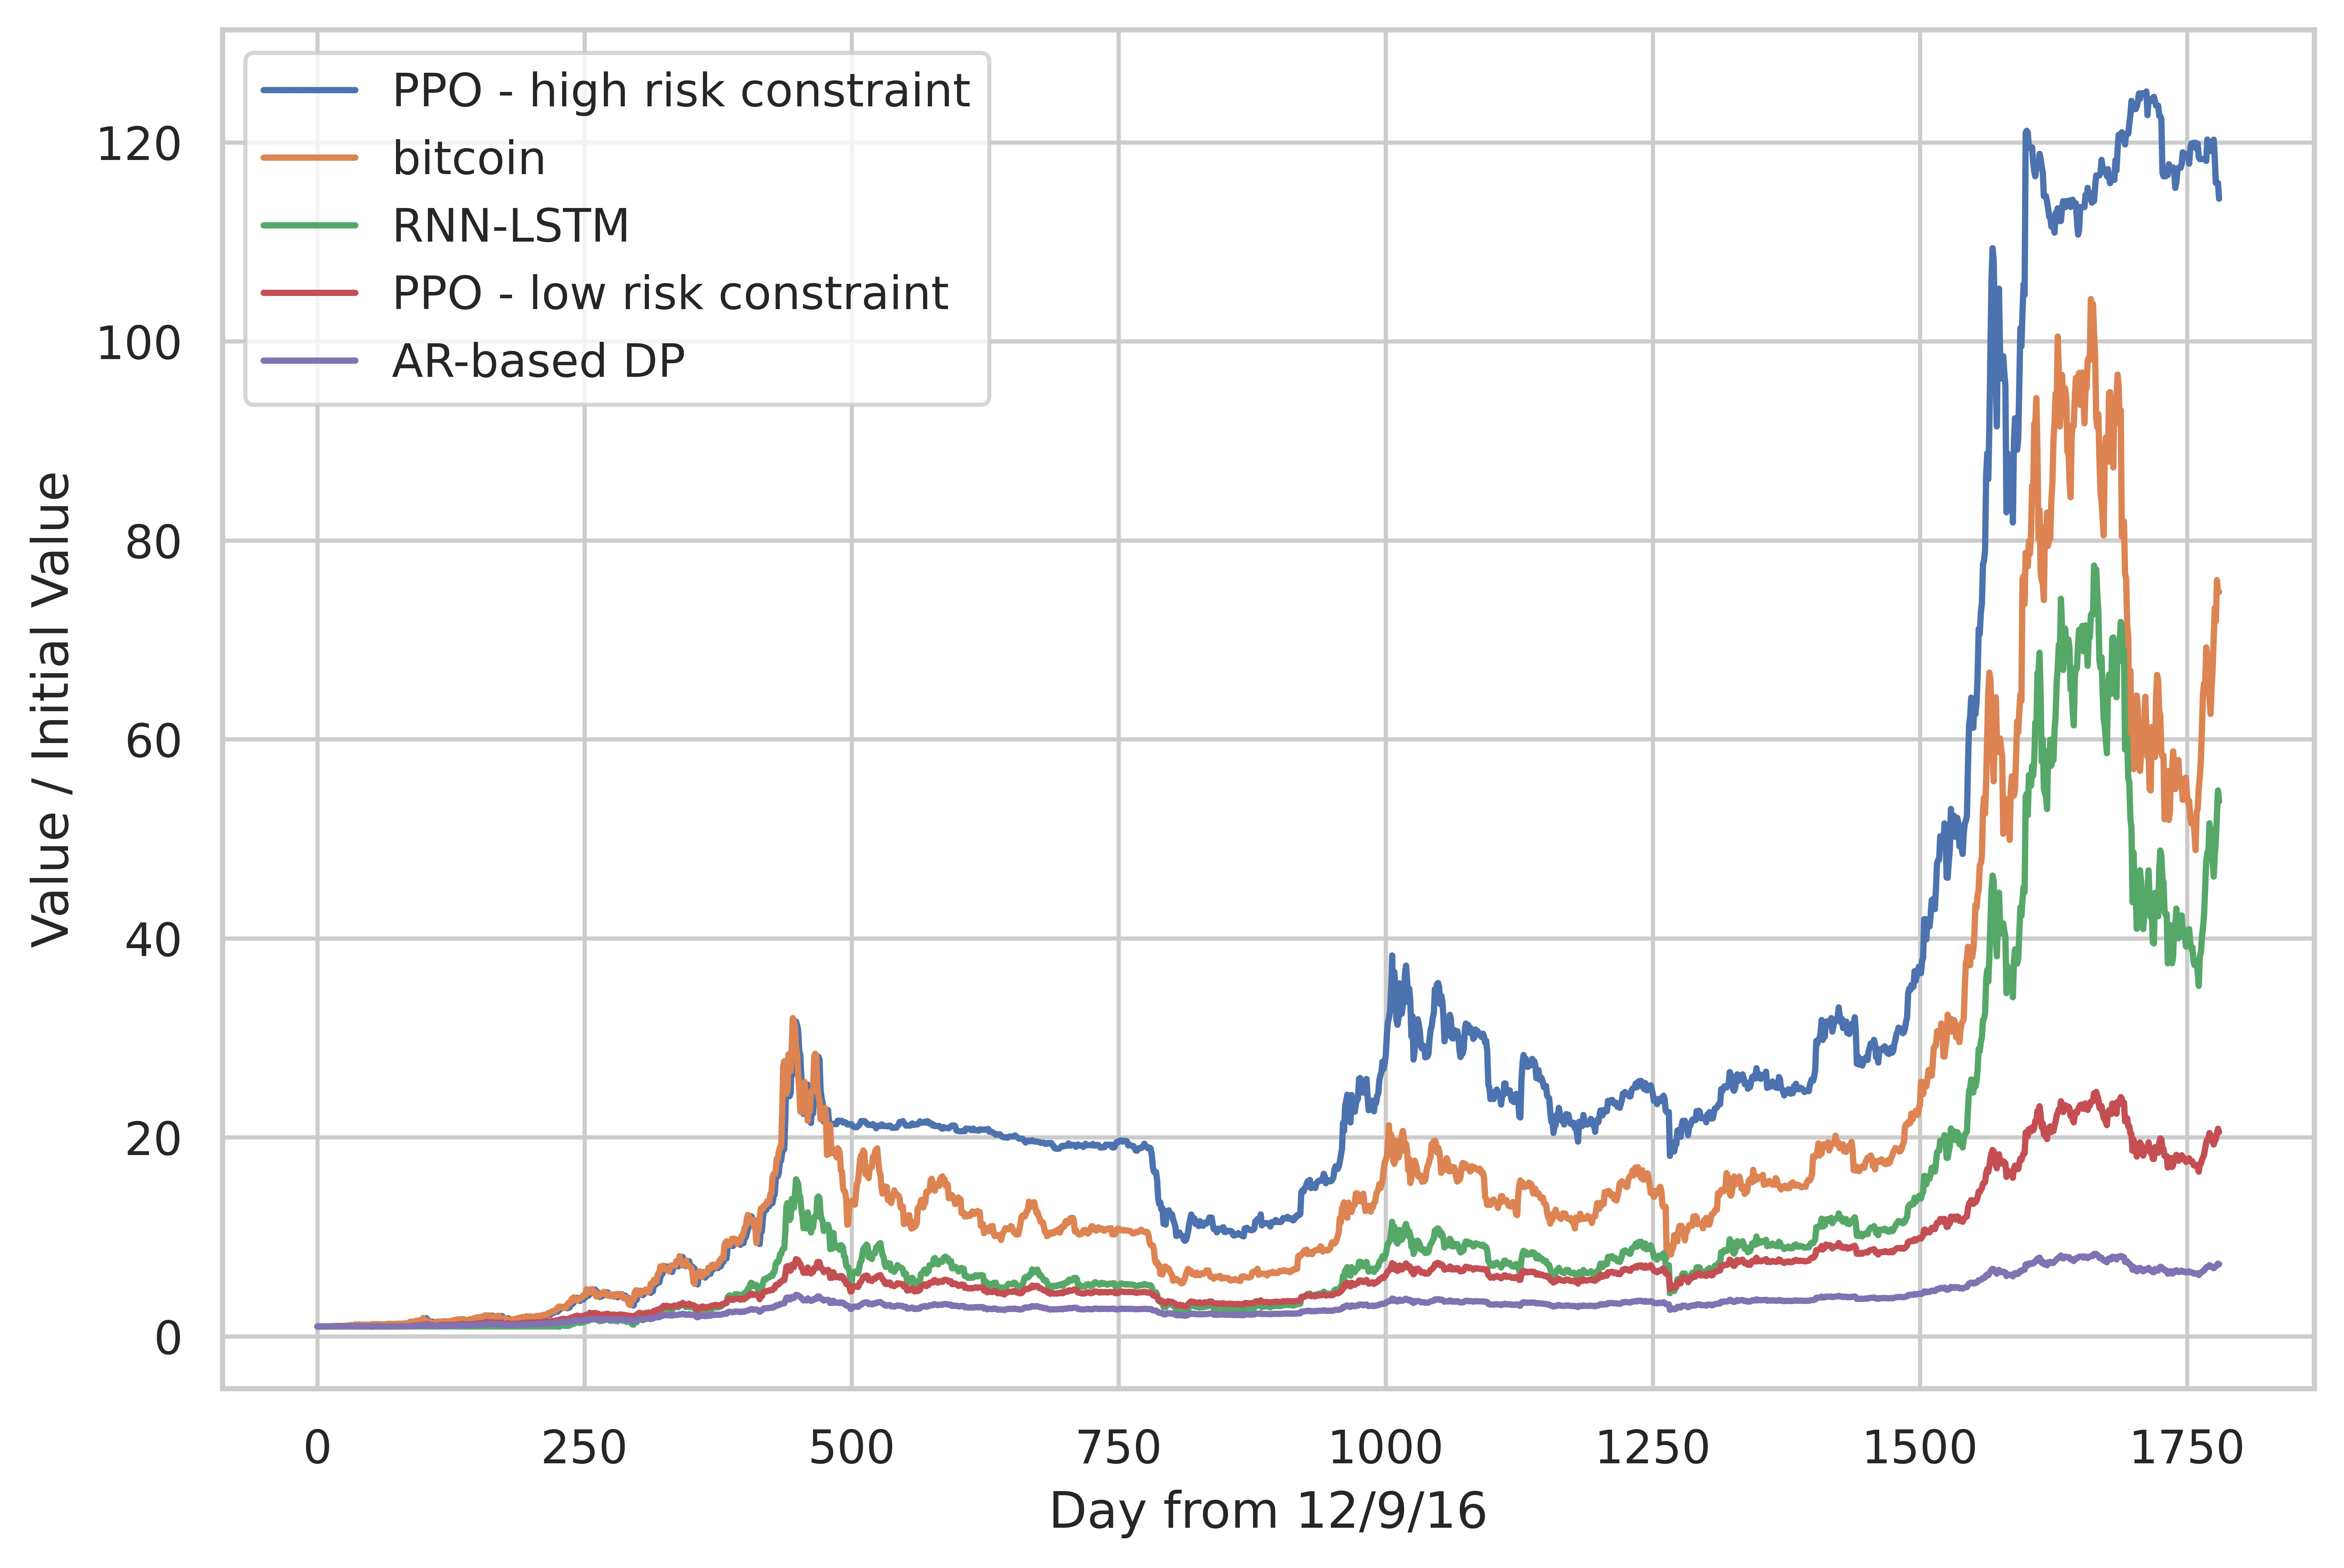
\includegraphics[width=10cm]{RL-final.jpg}
  \caption{Reinforcement learning results} \label{RL-Results}
\end{figure}

Proximal policy optimization with high risk constraint works the best among all the algorithms, with an acceptable amount of risk and high profit. PPO with low risk constraint works well when control of risk is a priority, with smaller but consistently growing returns that are less affected by the price of bitcoin. Both RNN-LSTM and Autoregression model performed relatively poorly, with the former being too risky and the latter too low rewarding.

The actions made the agent in the face of changes in the price of Bitcoin have a significant impact on its outcome.
Figure \ref{BTC} shows the number of \textit{units} of bitcoin bought by the agent against price changes in bitcoin with the PPO algorithm.

\begin{figure}[h]
  \small
  \centering
  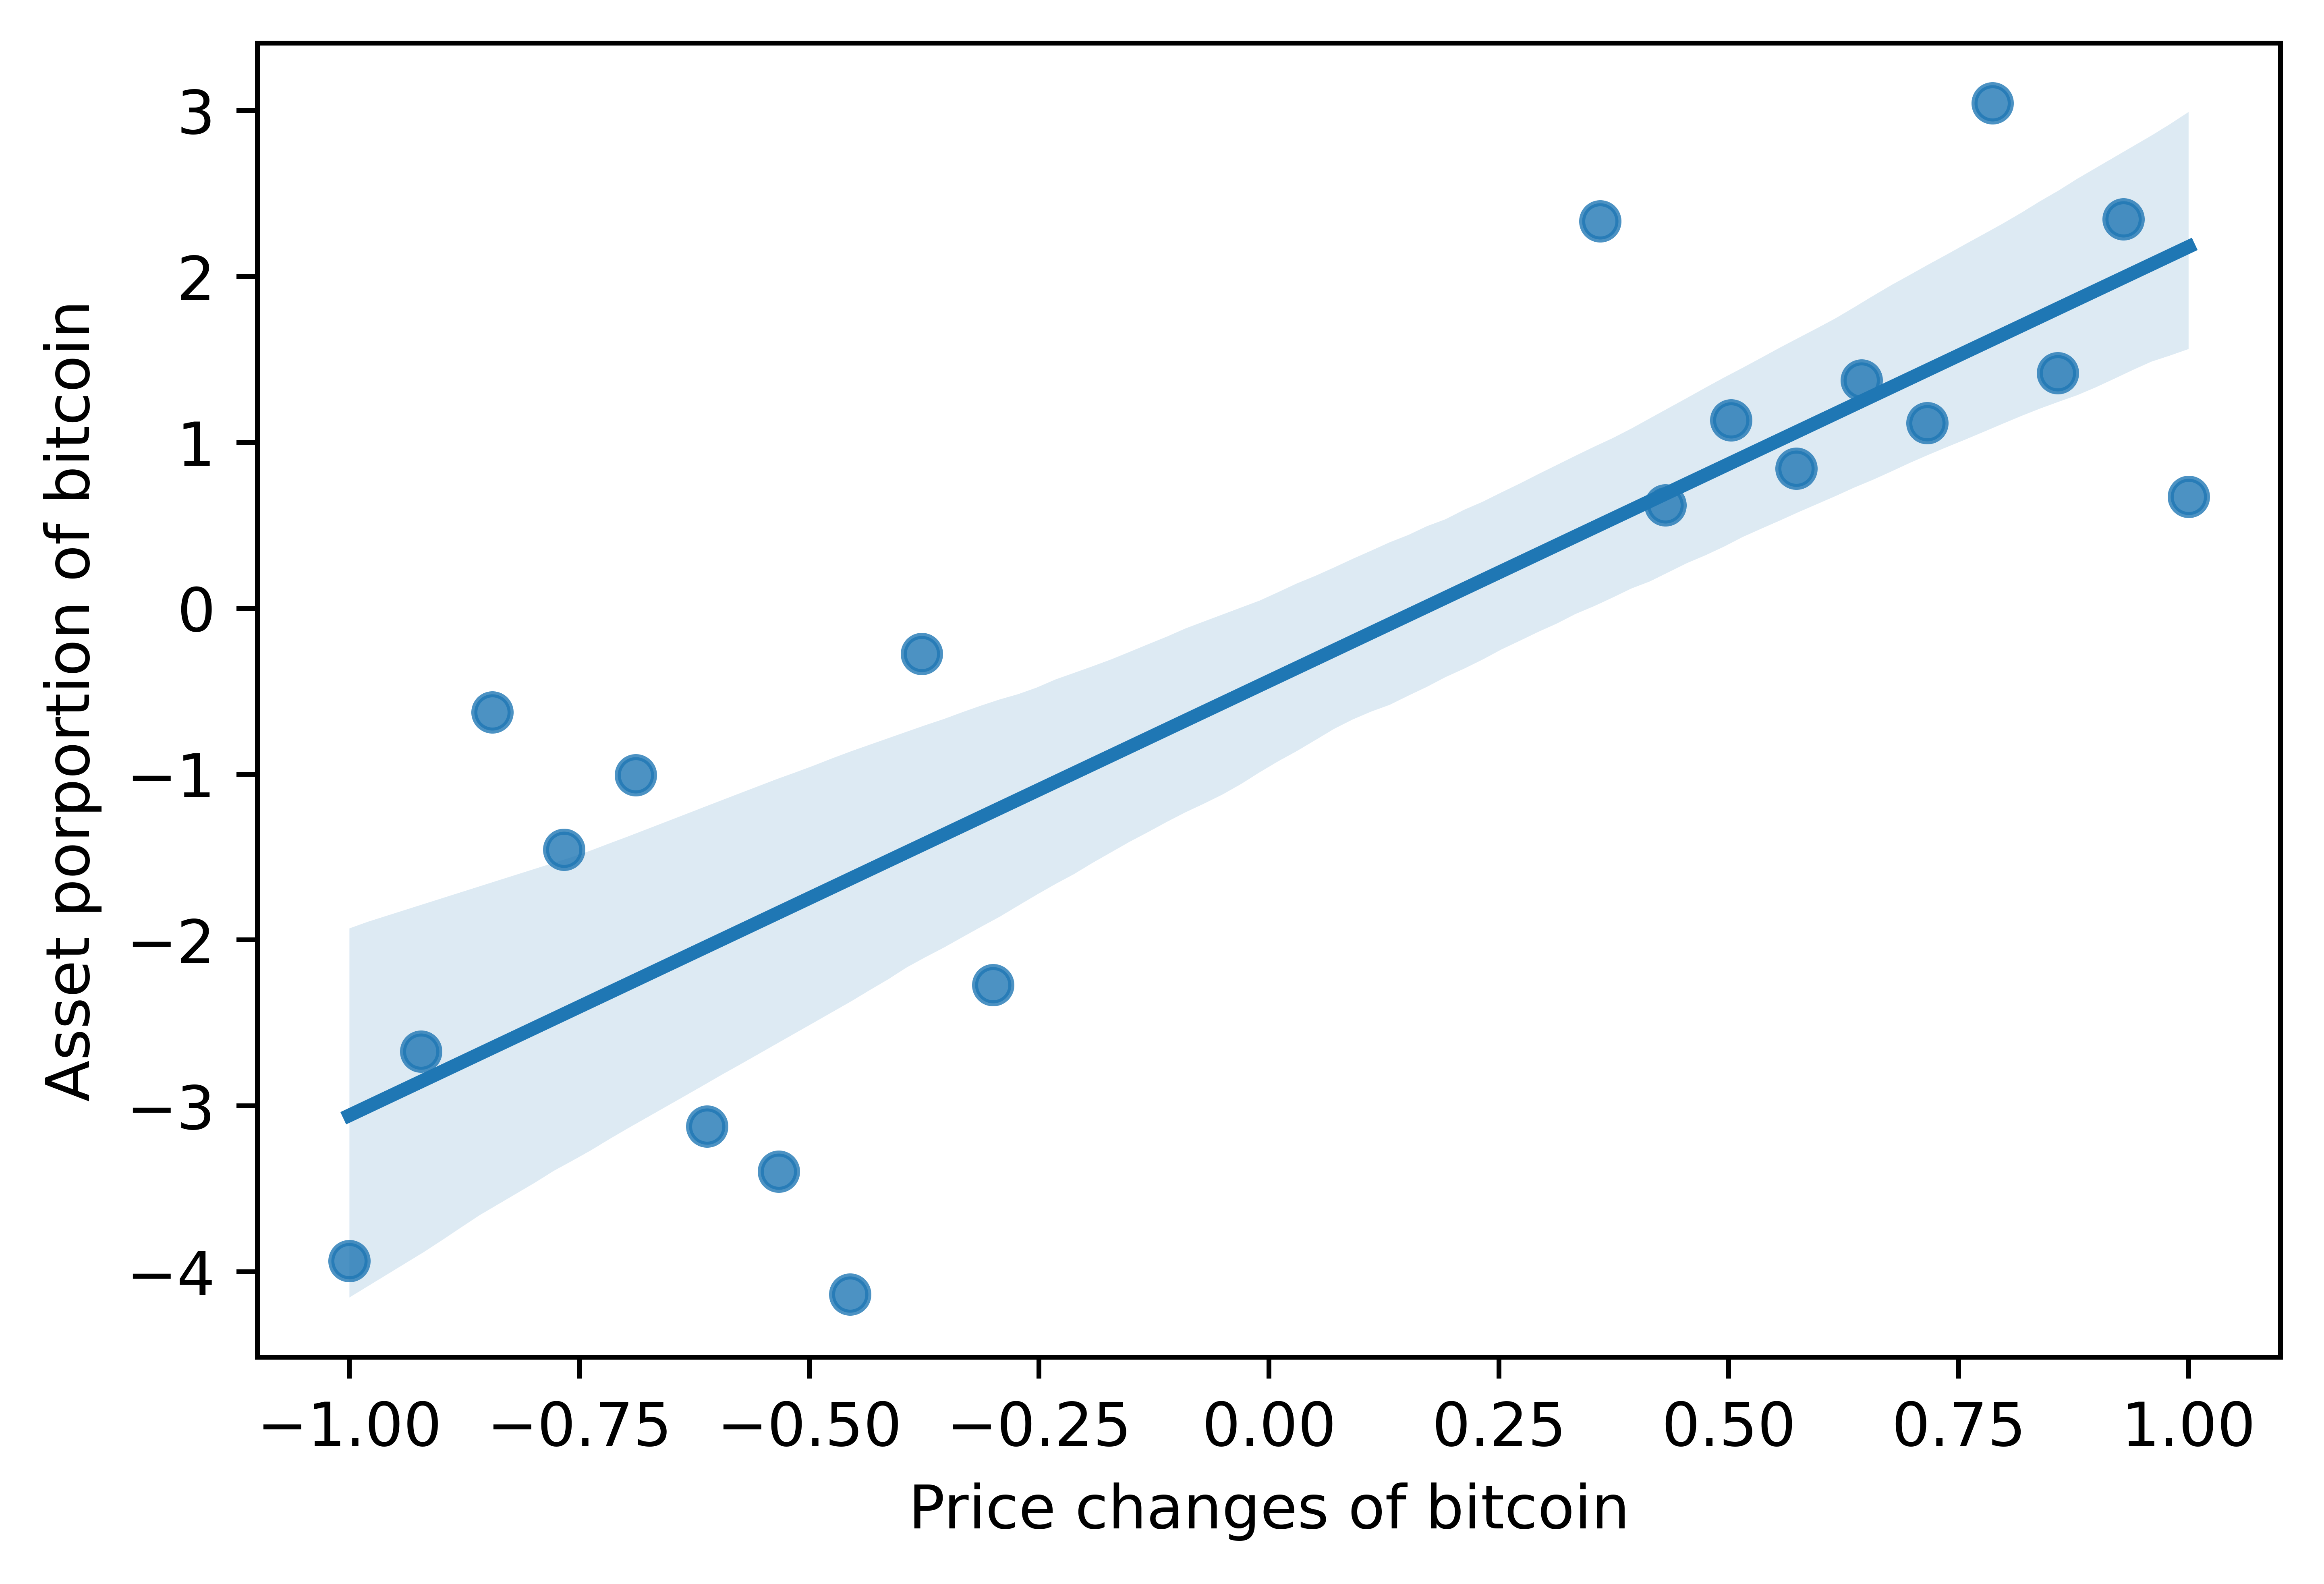
\includegraphics[width=10cm]{bitcoin.png}
  \caption{Agent behavior against price changes of BTC} \label{BTC}
\end{figure}

Each point in the figure stands for one actual transaction made by the agent.
The x-axis represents the average changes in price in the next 15 days.
The y-axis represents the amount of purchases, with positive and negative values indicating buys and sells respectively.
When the agent believes that there will be a significant change in the price of Bitcoin, it will change its holdings accordingly.
As can be seen from the figure, the purchase volume and change in price can be approximately fitted into a linear relationship.
That is to say, amount of purchases are positively correlated with predicted price changes.

And finally, the value of the initial \$1000 is shown in table \ref{final-value}:

\begin{table}
  \centering
  \begin{tabular}{@{}lr@{}}
    \toprule
    Algorithm & Final value(\$) \\
    \midrule
    Proximal policy optimization (high risk) & 112 \\
    {\color{gray} All in bitcoin} & {\color{gray} 76} \\
    RNN-LSTM & 55 \\
    Proximal policy optimization (low risk) & 21 \\
    AR-based DP & 8 \\
    \bottomrule
  \end{tabular}
  \caption{Final value of funds}
  \label{final-value}
\end{table}

\section{Conclusions}
\lipsum[6]

\section{Strengths and weaknesses}
\lipsum[12]

\subsection{Strengths}
\begin{itemize}
\item \textbf{Applies widely}\\
This  system can be used for many types of airplanes, and it also
solves the interference during  the procedure of the boarding
airplane,as described above we can get to the  optimization
boarding time.We also know that all the service is automate.
\item \textbf{Improve the quality of the airport service}\\
Balancing the cost of the cost and the benefit, it will bring in
more convenient  for airport and passengers.It also saves many
human resources for the airline. \item \textbf{}
\end{itemize}

\subsection{Weaknesses}

% \begin{thebibliography}{99}
% \bibitem{1} D.~E. KNUTH   The \TeX{}book  the American
% Mathematical Society and Addison-Wesley
% Publishing Company , 1984-1986.
% \bibitem{2}Lamport, Leslie,  \LaTeX{}: `` A Document Preparation System '',
% Addison-Wesley Publishing Company, 1986.
% \bibitem{3}\url{https://www.latexstudio.net/}
% \end{thebibliography}

\bibliographystyle{unsrt} %规定了参考文献的格式
\begin{center}
\bibliography{reference} %调出LaTeX生成参考文献列表
\end{center}

\begin{appendices}

\section{First appendix}

In addition, your report must include a letter to the Chief Financial Officer (CFO) of the Goodgrant Foundation, Mr. Alpha Chiang, that describes the optimal investment strategy, your modeling approach and major results, and a brief discussion of your proposed concept of a return-on-investment (ROI). This letter should be no more than two pages in length.

\begin{letter}{Dear, Mr. Alpha Chiang}

\lipsum[1-2]

\vspace{\parskip}

Sincerely yours,

Your friends

\end{letter}
Here are simulation programmes we used in our model as follow.\\

\textbf{\textcolor[rgb]{0.98,0.00,0.00}{Input matlab source:}}
\lstinputlisting[language=Matlab]{./code/mcmthesis-matlab1.m}

\section{Second appendix}

some more text \textcolor[rgb]{0.98,0.00,0.00}{\textbf{Input C++ source:}}
\lstinputlisting[language=C++]{./code/mcmthesis-sudoku.cpp}

\lstinputlisting[language=python]{./code/Harbin.py}

\section{Third appendix}

When you need to insert a table, use this template.

\begin{table}
\centering
\begin{tabular}{@{}lr@{}}
  \toprule
  Algorithm & Final value(\$) \\
  \midrule
  Proximal policy optimization (high risk) & 112 \\
  {\color{gray} All in bitcoin} & {\color{gray} 76} \\
  RNN-LSTM & 55 \\
  Proximal policy optimization (low risk) & 21 \\
  AR-based DP & 8 \\
  \bottomrule
\end{tabular}
\caption{Final value of funds}
\label{final-value123}
\end{table}

\end{appendices}
\end{document}
%%
%% This work consists of these files mcmthesis.dtx,
%%                                   figures/ and
%%                                   code/,
%% and the derived files             mcmthesis.cls,
%%                                   mcmthesis-demo.tex,
%%                                   README,
%%                                   LICENSE,
%%                                   mcmthesis.pdf and
%%                                   mcmthesis-demo.pdf.
%%
%% End of file `mcmthesis-demo.tex'.

